% Generated by plsimcount.pfseeds -- do not edit; regenerate instead.
% figure: B-order4-by-formula -- Every order-4 formula at measured r; median over seeds [1, 2, 3, 4, 5], bars = min..max
% metric=cnot gatebase=cz merged
% seed 1: git_commit=04cd66abb614bdc66fb48e891cef085a299e0ab1 git_dirty=False
% seed 2: git_commit=04cd66abb614bdc66fb48e891cef085a299e0ab1 git_dirty=False
% seed 3: git_commit=04cd66abb614bdc66fb48e891cef085a299e0ab1 git_dirty=False
% seed 4: git_commit=04cd66abb614bdc66fb48e891cef085a299e0ab1 git_dirty=False
% seed 5: git_commit=04cd66abb614bdc66fb48e891cef085a299e0ab1 git_dirty=False
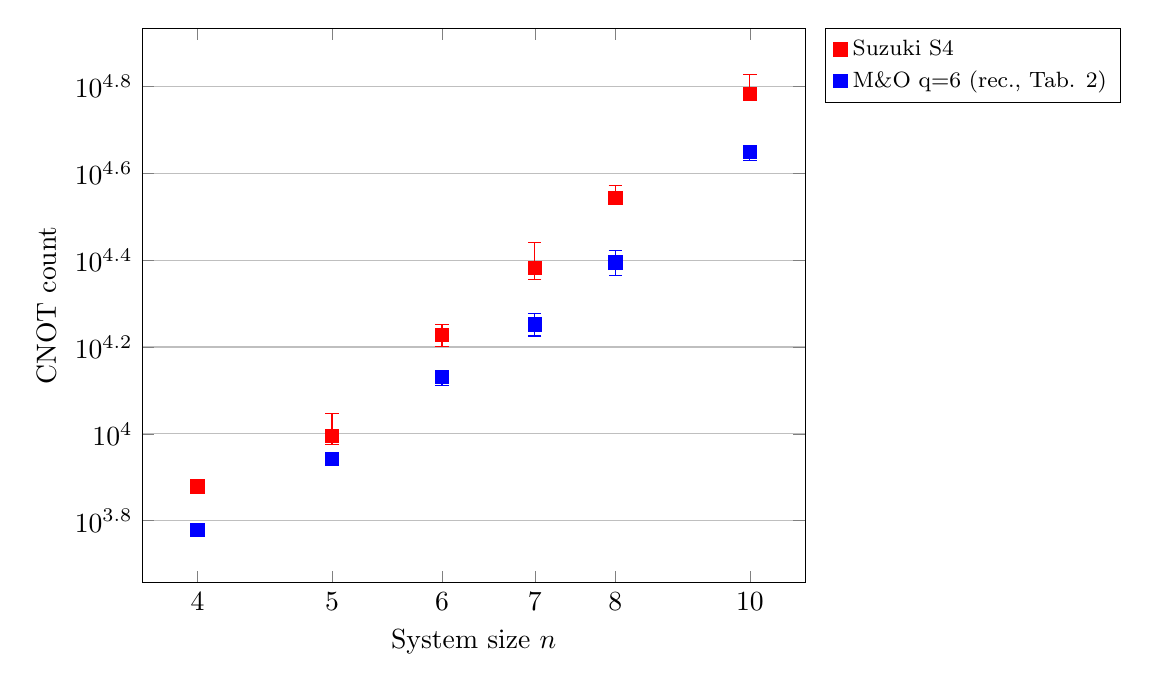
\begin{tikzpicture}
  \begin{loglogaxis}[
    width=10cm,
    xlabel={System size $n$},
    ylabel={CNOT count},
    xtick={4,5,6,7,8,10},
    xticklabels={4,5,6,7,8,10},
    ymajorgrids=true,
    legend pos=outer north east,
    legend cell align=left,
    legend style={font=\footnotesize},
  ]
    \addplot[only marks, red, mark=square*, mark size=2.4pt, mark options={solid, fill=red}, error bars/.cd, y dir=both, y explicit, error bar style={red}] coordinates {
      (4,7560) += (0,168) -= (0,168)
      (5,9870) += (0,1260) -= (0,420)
      (6,16884) += (0,1008) -= (0,1008)
      (7,24108) += (0,3528) -= (0,1470)
      (8,34944) += (0,2352) -= (0,1008)
      (10,60480) += (0,6720) -= (0,1680)
    };
    \addlegendentry{Suzuki S4}
    \addplot[only marks, blue, mark=square*, mark size=2.4pt, mark options={solid, fill=blue}, error bars/.cd, y dir=both, y explicit, error bar style={blue}] coordinates {
      (4,6000) += (0,0) -= (0,200)
      (5,8750) += (0,0) -= (0,0)
      (6,13500) += (0,0) -= (0,600)
      (7,17850) += (0,1050) -= (0,1050)
      (8,24800) += (0,1600) -= (0,1600)
      (10,44500) += (0,500) -= (0,2000)
    };
    \addlegendentry{M\&O q=6 (rec., Tab. 2)}
  \end{loglogaxis}
\end{tikzpicture}
